%!TEX root = ../main.tex

\section{Distribution-Aware Dataset Search}
\label{sec:problem}

We formalize the problem of distribution-aware dataset search over decentralized data repositories and discuss its research challenges.

\subsection{Problem Definition}
\label{sec:problem_definition}

Figure~\ref{fig:problem_overview} provides a semantic overview of the distribution-aware dataset search setting.
Based on the data market terminology by \textcite{asudeh_towards_2022}, we consider the passive-provider model, where data owners provide information about their datasets to search engines, and users come to a search engine to find relevant datasets.
We assume that users have complex search needs consisting of multiple requirements about the data they seek.
Specifically, we focus on distributional requirements.
In the following, we introduce our query model and formalize the search problem.

\paragraph{Predicate}
We model a user's search query as a Boolean predicate that can be checked with respect to any dataset or its corresponding profile.
Specifically, we consider \emph{keyword-based predicates}, denoted by $\cK_w(D)$, that hold when $D$'s profile contains the specified keyword $w$.
For example, the predicate ``\textit{title} = `census' '' returns true for all datasets whose title field contains ``census''.
In contrast, the simpler predicate ``cancer'' returns true whenever the word ``cancer'' appears anywhere in the dataset profile.
To enable distribution-aware dataset search, we additionally consider percentile predicates.

A \emph{percentile predicate} specifies the condition for a specific distributional requirement.
We define the predicate using the notions of \emph{column identifier} $C$, \emph{fraction} $ 0 < p \leq 1$, \emph{comparison operator} $\theta \in \sset {<, \leq, >, \geq}$, and \emph{range} $r \equiv [r_l, r_h)$, where $r_l, r_h \in \bR$ and $r_l < r_h$.
For a given $C$, $p$, $\theta$, and $r$, the predicate $\cP_{C, p, \theta, r}(D)$ defined on a dataset $D$ holds whenever the dataset contains a column matched by $C$ and the comparison $p \: \theta \: f$ is true, where $f$ is the fraction of values in the column that lie within the range $[r_l, r_h)$.
Other range definitions are possible but omitted for the sake of brevity.
More formally:
\[
\cP_{C, p, \theta, r}(D) \coloneq
\begin{cases}
    \true   & \text{if } \exists D[i]: \\
            & (D[i] \in C) \land \left(p \; \theta \; \frac{|\{x: x\in D[i] \land x\in [r_l,r_h)\}|}{|D[i]|}\right) \\
    \false  & \text{otherwise}
\end{cases}
\]
The column identifier $C$ can be a simple string or a more complex operation, such as a column match based on semantic similarity~\cite{zhang_ad_2018}.
In simple words, the predicate $\cP_{\text{age},0.5,\leq,[0,60)}(D)$ holds if \textit{``dataset $D$ has a column `age' and at least 50\% of the people are younger than 60''}.
However, a key challenge of evaluating percentile predicates over decentralized data repositories is that the search engine only has access to dataset profiles instead of raw data.
Therefore, we must design solutions capable of evaluating $\cP(P_D)$ rather than $\cP(D)$.\looseness=-1


\begin{table}[t]
    % NOTE: We place the table here to show it at a more convenient location in the text.
    \centering
    \footnotesize
    \caption{Notation overview.}
    \label{tab:notation_overview}
    \addtolength{\tabcolsep}{-0.5em}
    \begin{tabular}{cl cl cl}
        \toprule
        Symbol & Meaning                & Symbol  & Meaning            & Symbol & Meaning \\
        \midrule
        $D$    & Dataset                & $b$     & Histogram bin      & $n$    & \#~histograms \\
        $\cD$  & Dataset collection     & $c$     & Cluster            & $\cI$  & \system{} index \\
        $P_D$  & Dataset profile of $D$ & $k$     & \#~clusters        & $Q$    & Query \\
        $H$    & Histogram              & $\cB$   & Bin budget         & $\cK$  & Keyword pred. \\
        $H'$   & Aligned histogram      & $\cB_c$ & Bin budget for $c$ & $\cP$  & Percentile pred. \\
        $\cH$  & Histogram collection   & $\cH_c$ & Histograms in $c$  & $S$    & Result set \\
        \bottomrule
    \end{tabular}
\end{table}

\paragraph{Query}
A query $Q$ is a Boolean combination of keyword and percentile predicates.
Keyword-based dataset search has been extensively studied in the literature~\cite{chapman_dataset_2020, noy_google_2019, wei_survey_2013, zhang_ad_2018}.
Here, we focus on supporting distribution-aware search with $Q(D) \equiv \cP(D)$.

We now define the distribution-aware dataset search problem.

\begin{problem}[\textsc{Distribution-Aware Dataset Search}]
    Given a collection of data sources $\cS$, such that each source $s$ has a data repository $\cD_s = \sset{D_1,\dots, D_d}$ and shares corresponding dataset profiles $\cM_s = \sset{P_{D_1},\dots, P_{D_d}}$, and a dataset search query $Q$, find the set of datasets $S = \sset{D: D\in \cD \text{ and } Q(P_D)\text{ holds}}$.
\end{problem}

\subsection{Research Challenges}
\label{sec:research_challenges}

Of the three challenges presented in Section~\ref{sec:intro}, we address C1 by using histograms and C2 by proposing percentile predicates.
We now discuss the difficulties of designing a fast and accurate solution for evaluating percentile predicates on histograms~(C3).
Across all stakeholders, the desiderata for a distribution-aware dataset search engine are: (1)~interactive query execution time with sublinear scaling in the number of datasets, (2)~accurate results, and (3)~a minimal resource (i.e.,~memory) footprint of any data structures other than dataset profiles.
These three dimensions form a triangle with a performance trade-off since we cannot maximize all dimensions simultaneously: producing accurate results in minimal time requires precomputation, which implies higher memory usage; accurate results without additional memory usage require an iterative execution with linear runtime; and returning results in sublinear time with minimal memory usage effectively means guessing with arbitrary accuracy.
Therefore, at least one dimension will always perform worse than if we solely optimized a solution for it.
Beyond this trade-off, a central challenge of our problem is the handling of heterogeneous histograms provided by the data owners.

\paragraph{Predicate Evaluation With Histograms}
In principle, evaluating a percentile predicate using a histogram $H$ is straightforward, as its bin edges and densities include the required information.
Consider the exemplary histograms from Figure~\ref{fig:example_histograms_1} and our predicate $\cP_{\text{age}, 0.5, \leq, [0, 60)}$, looking for datasets where at least 50\% of the people are younger than 60.
To evaluate it, we sum up the density $f$ of all bins that fall into $[r_l, r_h)$.
For $H_a$, we have $f=0.6$; thus, the predicate holds.
Likewise, it is straightforward to see that $\cP$ does not hold for $H_b$.
Yet, the triviality of this example does not extend to decentralized data repositories, as each data provider independently creates histograms of their data at will so that a bin may only partially overlap with $[r_l, r_h)$, such as in the case of histogram $H_c$.\looseness=-1

Evaluating a predicate on heterogeneous histograms often requires estimating a bin's contribution to $f$.
There are several intra-bin value distribution estimation strategies~\cite{cormode_synopses_2011}.
Common strategies are to underestimate (ignore bin $b$), overestimate (add the total density of $b$), or assume a continuous value distribution and add a share of $b$'s density proportional to the overlap with range $r$.
Unless we overestimate $f$ for $\theta =$``<'' and underestimate it for $\theta =$``>'', we risk filtering out dataset columns that match the predicate.
Since a histogram is a lossy representation of $D$, this approach may produce false positives (a limitation of synopsis-based dataset search).
However, the approach guarantees full recall, a crucial requirement to ensure effectiveness.
If full recall is not required, the estimation could be changed to achieve full precision or to maximize $F_1$ score.

\begin{figure}[t]
    \centering
    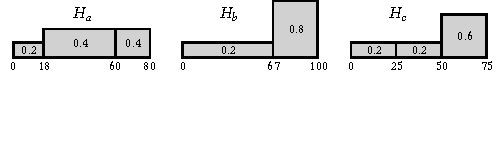
\includegraphics[trim=0 1.35cm 0 0]{figures/diagrams/example_histograms.pdf}
    \caption{Histograms $\boldsymbol{H_a}$, $\boldsymbol{H_b}$, and $\boldsymbol{H_c}$.}
    \Description{Three exemplary histograms to underscore research challenges.}
    \label{fig:example_histograms_1}
    % Max width: 241.14749pt / 8.47cm
\end{figure}

\paragraph{Predicate Evaluation Over Dataset Collections}
A simple yet effective way to evaluate a percentile predicate at the dataset collection level is a technique we call \pscan.
It iterates through each histogram $H$, determines the bins that fall into the range $r$, and adds $H$ to the result set $S$ if the predicate is fulfilled.
This makes it an accurate and memory-efficient solution, as it uses no additional data structures.
However, a major limitation is that it scales linearly in the number of histograms.
Even though \pscan can filter the histogram collection based on column identifier $C$, a significant number of histograms can remain after filtering.
For example, Kaggle~\cite{kaggle_inc_kaggle_2024} has more than $15\:000$ datasets that match the keyword ``age'' and more than $23\:000$ datasets matching the query ``date'' as of February 2024.
This problem becomes exacerbated if users pose generic column identifier predicates instead of keywords, such as \textit{``match any column related to finance''}.
Thus, \pscan leaves a need for a fast and accurate as well as a fast and resource-efficient solution, which we address in this paper.

% Practical problems
The critical problem for the sublinear scalability of percentile predicate evaluation is the heterogeneity of histograms from decentralized data repositories.
As the histograms have different numbers and distributions of bins, we must individually identify the bins within a predicate's range per histogram.
Allowing arbitrary value ranges in a predicate further complicates the problem since an infinitely large number of possible ranges must be considered for an index.
If we instead require that either $r_l = -\infty$ or $r_h = \infty$, we can achieve orders of magnitude speedups for percentile predicates with intelligent precomputation.
Such ``one-sided'' intervals for specifying a range enable us to execute queries similar to the ones in our motivating example.
Assuming that $r_l = -\infty$ or $r_h = \infty$, the range $r$ of a predicate effectively cuts the number line into two parts.
Consequently, we can rewrite any predicate with $r_l = -\infty$ into a predicate with $r_h = \infty$ (and vice versa) by setting $r_l = r_h$, replacing $p$ with $1-p$ and flipping the comparison operator $\theta$.
Without loss of generality, we therefore assume $r_l = -\infty$ and simplify the notation of a percentile predicate to $\cP_{C, p, \theta, r_h}(P_D)$ for the rest of this paper.
